
\chapter{Model of Solution System\label{chpt:models}}

Computing models of solvents are broadly divided into two types: those
treating the solvent as a continuous medium (implicit models) and
those describing the individual solvent molecules (explicit models).
In the continuum model, the solvent is characterized only by the dielectric
constant $\varepsilon$ and contains an artificial-shaped cavity.
The explicit models can have more specific scales. Within the scope
of classical mechanics, the solvent molecules are often described
as rigid entities carrying distributed point charges; the most expensive
methods involves flexible and polarizable explicit models. In computational
chemistry, less precise models often have wider usage (the so-called
coarse-grained models; for example, the proteins are treated in the
unity of residues). As the theory of liquids was firstly established
for spherical atom-like solvent particles, the model adopted by such
theory is a rigid molecule model, only depending on its position and
orientation, i. e. there is no relative movement within the solvent
particles. This approximation has been proven reasonable \citep{Gray-Gubbins}.
In this section, we will give a brief introduction of the implicit
model in order to facilitate later discussion on solvation free energy
corrections. \textcolor{red}{We will then focus on the rigid solvent
models and discuss the limits of each approximation.} The flexible
and polarizable models will also be briefly mentioned.


\section{Continuum solvation models}

Continuum models \citep{Jensen,Cramer_1999,Tomasi_1994_implicit_model},
which are popular in QM calculations, consider the solvent as a uniform
polarizable medium with dielectric constant $\varepsilon$\marginpar{The dielectric constant $\varepsilon$ is the only parameter characterizing
the solvent. It is normally a constant value, but it can depend on
the distance from the solute $M$. (see $\mathsection$\ref{sub:Poisson=002013Boltzmann-methods})}, with the solute $M$ placed in the cavity within this medium (figure
\ref{fig:Reaction-field-model}) 

\begin{figure}[h]
\begin{centering}
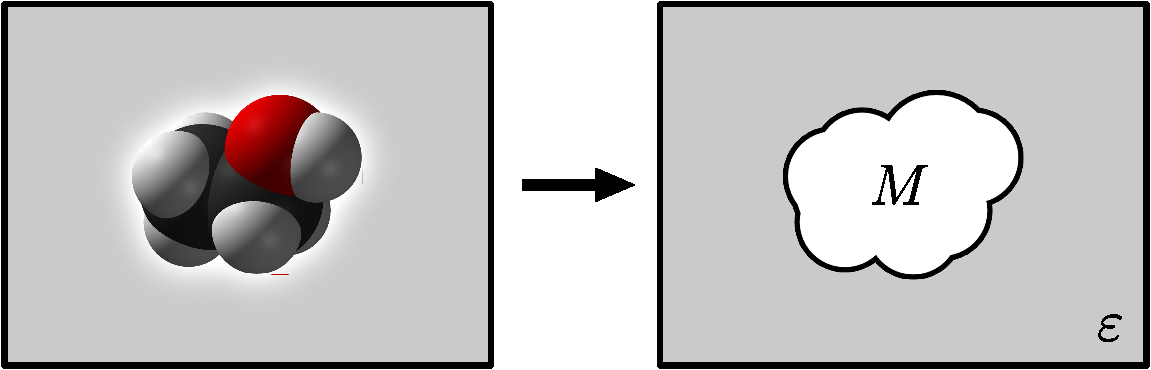
\includegraphics[width=0.72\columnwidth]{_figure/reaction-field-model_2}
\par\end{centering}

\caption{Continuum solvent model\label{fig:Reaction-field-model}}
\end{figure}


The solvation Gibbs free energy according to this model is
\begin{equation}
\Delta G_{\mathrm{solvation}}=\Delta G_{\mathrm{cavity}}+\Delta G_{\mathrm{dispersion}}+\Delta G_{\mathrm{elec}}\label{eq:cm}
\end{equation}
where $\Delta G_{\mathrm{cavity}}>0$ is the energy needed to create
a hole in the medium, and $\Delta G_{\mathrm{dispersion}}$ is the
dispersion interaction, which is roughly the van der Waals energy
$\Delta G_{\mathrm{vdW}}<0$ between the solvent and solute. In principle,
there may also be a repulsive component, and the dispersion term is
sometimes denoted dispersion / repulsion. $\Delta G_{\mathrm{elec}}<0$
is the contribution of electrostatic interactions, introduced by electric
charge distribution of $M$ which polarizes the medium, and the action
back of the medium on the molecule (reaction field). 

The initial two terms in eq. (\ref{eq:cm}) may be linked to the configuration
of the first solvation shell (cavity). The definition of cavity varies
from the simplest sphere or ellipsoid to the surface of the ensemble
atomic surfaces defined by the van der Waals radii in the solute.
It's somehow reasonable to consider the cavity area proportional to
the number of solvent molecules in the first solvation shell. This
number can be calculated as the area passing through the middle region
of first shell solvent. This area, named as the solvent-accessible
surface area (SASA) \citep{SAS_1,SAS_2}, can be calculated by adding
the radius of the probe solvent ball on the solvent excluded surface
area (figure \ref{fig:sasa}).

\begin{figure}[h]
\begin{centering}
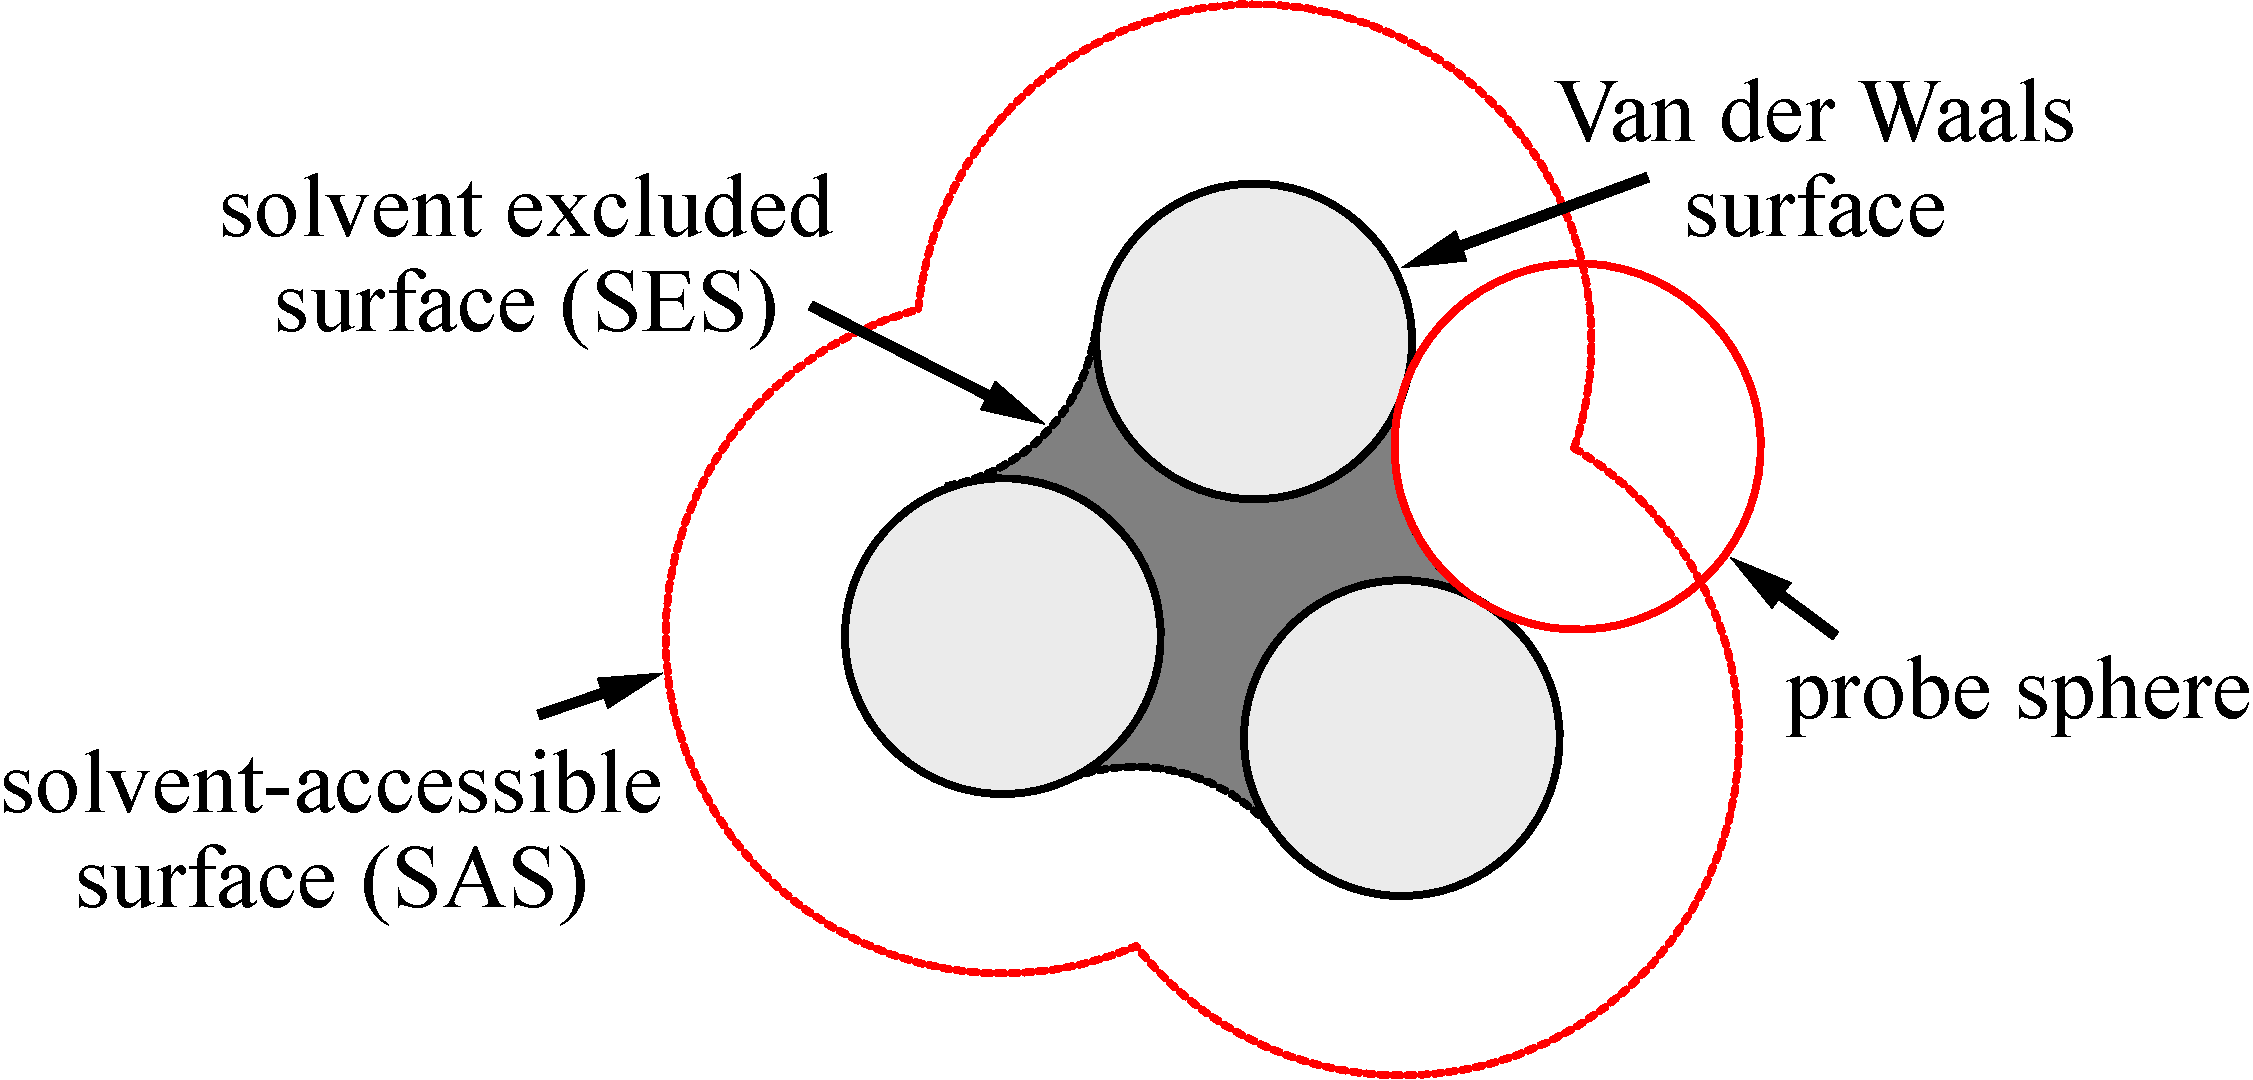
\includegraphics[width=0.55\columnwidth]{_figure/SASA}
\par\end{centering}

\caption[Definition of cavity surfaces]{Definition of cavity surfaces\label{fig:sasa}. The solvent accessible
surface (SAS) traced out by the center of the probe representing a
solvent molecule. The solvent excluded surface (SES) is the topological
boundary of the union of all possible probes that do not overlap with
the molecule.}
\end{figure}


The energy required to create such a cavity and the stabilization
due to van der Waals interactions between the solute and solvent,
assumed to be proportional to the surface area of the cavity, is expressed
as
\begin{equation}
\Delta G_{\mathrm{cavity}}+\Delta G_{\mathrm{dispersion}}=\gamma S_{\mathrm{SASA}}+\beta
\end{equation}
or parameterized by having a constant $\xi$ specific for each atom
type, with the $\xi$ parameters being determined by fitting to experimental
solvation data:
\begin{equation}
\Delta G_{\mathrm{cavity}}+\Delta G_{\mathrm{dispersion}}=\sum_{i}^{\mathrm{atoms}}\xi_{i}S_{i}
\end{equation}


The models and methods to calculate the electrostatic contribution
$\Delta G_{\mathrm{elec}}$ have varied greatly according to their
usage. The sections below list the most common examples. By the way,
the integration of continuum models into \acs{QM} calculations is
also important, which will not be detailed as it does not link to
our theory. Such kind of methods are called the self-consistent reaction
field (SCRF) models, which treat the calculation of the solute-solvent
interaction in addition to the solute wave function by an iterative
procedure. Some examples are presented in the list of Gaussian keyword
SCRF \citep{scrf}, and well reviewed by for example Tomasi \citep{Tomasi_1994_implicit_model,tomasi_quantum_2005}
and Jensen \citep{Jensen}.


\subsection{Poisson-Boltzmann methods\label{sub:Poisson=002013Boltzmann-methods}}

The Poisson-Boltzmann equation (PBE) \citep{holst_1994_poisson} permits
to calculate the electrostatic potential $V_{\mathrm{elec}}$ in the
continuum model, such that the electrostatic component of the free
energy can be written as
\begin{equation}
\Delta G_{\mathrm{elec}}=\frac{1}{2}\int\mathrm{d}\mathbf{r}\rho_{q}(\mathbf{r})V_{\mathrm{elec}}(\mathbf{r})
\end{equation}
where $\rho_{q}$ is the charge distribution of the continuous medium.

The Maxwell-Gauss equation in SI units convention gives 
\begin{equation}
\nabla\cdot D(\mathbf{r})=\dfrac{\rho_{q}(\mathbf{r})}{\varepsilon_{0}}
\end{equation}
where $D(\mathbf{r})=\varepsilon_{0}E(\mathbf{r})+P(\mathbf{r})$
is the electric displacement field, $P(\mathbf{r})$ is the system
polarization, $E(\mathbf{r})$ the electric field, $\varepsilon_{0}$
the vacuum permittivity. $D(\mathbf{r})$ can also be expressed in
term of the position-dependent dielectric constant $\varepsilon(\mathbf{r})$,
$D(\mathbf{r})=\varepsilon(\mathbf{r})E(\mathbf{r})$, thus gives
\begin{equation}
\nabla\cdot\varepsilon(\mathbf{r})E(\mathbf{r})=\dfrac{\rho_{q}(\mathbf{r})}{\varepsilon_{0}}
\end{equation}
or in terms of electrostatic potential 
\begin{equation}
\nabla\cdot\left[\varepsilon(\mathbf{r})\nabla V_{\mathrm{elec}}(\mathbf{r})\right]=-\dfrac{\rho_{q}(\mathbf{r})}{\varepsilon_{0}}\label{eq:poisson}
\end{equation}


This second-order differential equation (\ref{eq:poisson}) is called
the Poisson equation. 

This equation cannot be solved analytically for complex geometries
(such as protein), therefore, it is done numerically using numerical
methods. Such methods are mentioned in, for example, the article of
Roux and Simonson \citep{roux_implicit_1999} or Holst \citep{holst_1994_poisson}.
A density functional approach based on the minimization of the polarization
density can be equally used to solve this equation \citep{Marchi_2001,Levy_2005}.

If the solvent is ionic, the Poisson equation can be modified by taking
into account a (thermal) Boltzmann distribution of ions in the solvent,
leading to the Poisson-Boltzmann Equation:
\begin{equation}
\begin{array}{r}
\nabla\cdot(\varepsilon(\mathbf{r})\nabla\phi(\mathbf{r}))-\kappa^{2}\left(\dfrac{kT}{q}\right)\sinh\left(\dfrac{qV_{\mathrm{elec}}(\mathbf{r})}{kT}\right)=-\dfrac{\rho(\mathbf{r})}{\varepsilon_{0}}\\
\kappa^{2}=\dfrac{8\pi q^{2}I}{kT}
\end{array}
\end{equation}


Here $q$ is the ion charge, $I$ is the ion strength of the solution,
and \textcolor{red}{the $\kappa^{2}$ factor is inversely related
to the Debye-Hückel length. {[}Unity?{]}}


\subsection{Born / Onsager / Generalized Born models\label{sub:Born-/-Onsager}}

For simple geometries, the Poisson equation (\ref{eq:poisson}) can
be solved analytically.

The simplest model is a spherical cavity. For a net charge $q$ in
a cavity of radius $a$, the electrostatic free energy of a medium
with a dielectric constant of $\varepsilon$ is given by the Born
model: 

\begin{equation}
\Delta G_{\mathrm{elec}}(q)=-\dfrac{1}{8\pi\varepsilon_{0}}\left(1-\frac{1}{\varepsilon}\right)\frac{q^{2}}{2a}
\end{equation}


However, the Born model is not fully capable to predict the solvent
behavior in a lot of cases \citep{Jensen}. Other similar models include
Onsager model, in which a dipole point (characterized by momentum
$\mu$) is put in a spherical cavity; and the Kirkwood model refers
to a general multipole expansion in a spherical cavity; while the
Kirkwood-Westheimer model arises for an ellipsoidal cavity.

The generalized Born (GB) model is the superposition of several net
charges in spherical cavities as Born model describes, with a similar
formalism: \textcolor{red}{(Unity?)}
\begin{equation}
\Delta G_{\mathrm{elec}}=-\dfrac{1}{8\pi\varepsilon_{0}}\left(1-\frac{1}{\varepsilon}\right)\sum_{i}\sum_{j}\frac{q_{i}q_{j}}{f_{ij}}
\end{equation}
where the function $f_{ij}$ depends on the internuclear distance
and Born radii for each pair of atoms, $a_{i}$ and $a_{j}$:
\begin{equation}
f_{ij}=\sqrt{r_{ij}^{2}-a_{i}a_{j}\exp\left(\frac{r_{ij}^{2}}{4a_{i}a_{j}}\right)}
\end{equation}
$r_{ij}$ being the distance between the centers of atom $i$ and
$j$. 

The GB model provides a very fast method, with rather the same accuracy
compared to Poisson-Boltzmann calculations. That makes it widely used
to perform optimization and simulations.


\section{Model potential of explicit molecules}

The model potential frequently used in the theory of liquids is a
classical, rigid, pairwise additive model \citep{Hensen-McDonald,Gray-Gubbins}.
It is based on three assumptions. 
\begin{enumerate}
\item Firstly, the quantum effect of solvent should have been ignored. It
is assumed that the rotational and transitional motion of solvent
particles are continuous and classical, that means the separation
of both transitional and rotational states are largely inferior of
$k_{\mathrm{B}}T$. For light molecules, that is not always convincing.
Some molecules containing hydrogen (e. g. $\mathrm{H_{2}O}$, $\mathrm{NH_{3}}$,
and particularly $\mathrm{H_{2}}$) exhibit obvious quantum effects
at low temperature in liquid state. Gaseous $\mathrm{H_{2}O}$ and
$\mathrm{NH_{3}}$ also need quantum effect corrections. However,
in which we are interested the most, the liquid $\mathrm{H_{2}O}$
at room temperature, the contribution of this effect is enough small.
And obviously, there should not be any chemical interaction of solvent
with the solute.
\item Secondly,\marginpar{Compared to atomic models that only depend on $\mathbf{r}^{N}$, the
angular correlations can give influence on both structural and thermodynamics
proprieties. That is why our theory is extended to linear case ($\mathbf{\Omega}\equiv(\Theta,\Phi)$)
then molecular case ($\mathbf{\Omega}\equiv(\Theta,\Phi,\Psi)$ ).} the intramolecular movement (vibration and internal rotation) should
be either independent of transitional and rotational movement or absent.
This rigid molecule approximation assumes that the intermolecular
potential $\mathcal{U}(\mathbf{r}^{N},\mathbf{\Omega}^{N})$ only
depends on the positions of the $N$ molecular centers $\mathbf{r}^{N}\equiv\mathbf{r}_{1}\mathbf{r}_{2}\ldots\mathbf{r}_{N}$
and on their orientation $\mathbf{\Omega}^{N}$, where $\mathbf{\Omega}\equiv(\Theta,\Phi,\Psi)$
represents the Euler angles (figure \ref{fig:Euler-angles}).


\begin{figure}[h]
\begin{centering}
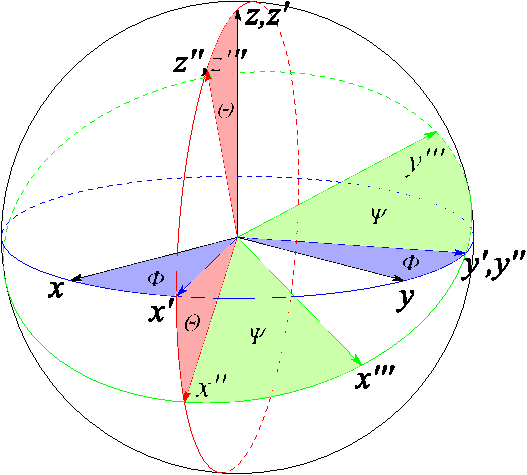
\includegraphics[scale=0.7]{_figure/euler_sphere}
\par\end{centering}

\caption[Euler angles]{Euler angles. The result basis vectors of the new orientation are
obtained by 3 sequential operations: (1) A rotation $\phi$ $(0<\phi<2\pi)$
about the $z$-axis, bringing the frame of axes from the initial position
$\mathbf{S}$ into the position $\mathbf{S}'$ (2) A rotation $\theta$
$(0<\theta<\pi)$ about the $y$-axis of the frame $\mathbf{S}'$,
which is transformed into $\mathbf{S}''$ (3) A rotation $\psi$ $(0<\psi<2\pi)$
about the $z$-axis of the frame $\mathbf{S}''$.\label{fig:Euler-angles}}
\end{figure}



\textcolor{red}{(The choice of molecular centre?)}


This approximation is quite realistic for molecules in which the separation
of vibrational states largely exceed $k_{\mathrm{B}}T$, \textcolor{red}{and}
implies that the solvent molecule stays in its ground vibrational
state. \textcolor{red}{(Why?)} For many small molecule solvents such
as $\mathrm{N_{2}}$, $\mathrm{CO_{2}}$, $\mathrm{C_{6}H_{6}}$,
it is the case, expect of water. \textcolor{red}{(...) The non-rigidity
of water should be studied in the cases of (...)}

\item Finally, the intermolecular forces have been assumed to be pairwise
additive:
\begin{equation}
\mathcal{U}(\mathbf{r}^{N},\mathbf{\Omega}^{N})=\frac{1}{2}\sum_{i\neq j}u(\mathbf{r}_{ij},\mathbf{\Omega_{i}},\mathbf{\Omega_{j}})=\sum_{i<j}u(\mathbf{r}_{ij},\mathbf{\Omega_{i}},\mathbf{\Omega_{j}})\label{eq:pair-potential}
\end{equation}
That means the model potential only depends on the intermolecular
separation $\mathbf{r}$ and on the molecular orientations $\mathbf{\Omega}_{1}$
and $\mathbf{\Omega}_{2}$. This approximation is quasi-exact for
low density gases, where the three and more body terms decrease rapidly,
but for dense fluids, in most of cases the multi-body potential can
not be ignored, but it is often taken into account by an effective
pair potential (measured by experiments or calculated by simulations)
due to computational cost. Three-body omission can cause surface tension
problem, \textcolor{red}{(...)}


The complete model potential with higher order corrections can be
written in the form of


\begin{equation}
\mathcal{U}(\mathbf{r}^{N},\mathbf{\Omega}^{N})=\sum_{i<j}u(ij)+\sum_{i<j<k}u(ijk)+\sum_{i<j<k<l}u(ijkl)+...
\end{equation}
where $u(ijk)=u(\mathbf{r}_{ij},\mathbf{r}_{jk},\mathbf{r}_{ki},\mathbf{\Omega_{i}},\mathbf{\Omega_{j}},\mathbf{\Omega_{k}})$.

\end{enumerate}
\textcolor{red}{For water, most of the publications have already shown...
at the approximation level in this thesis...}

In the test below we will present some common models from the most
simple to the most complicate.


\subsection{Interaction of spherical particle}

The simplest model of a fluid is the hard sphere model. With $d$
is the hard-sphere diameter, the pair potential
\begin{equation}
u(r)=\begin{cases}
\infty & r<d\\
0 & r>d
\end{cases}
\end{equation}
\textcolor{red}{This model can represent some physical systems, such
as ... }However, the absence of attractive force \textcolor{red}{...}
.

More realistic neutral particle models, like Lenard-Jones (LJ) model,
have a potential energy curve that has the same shape as the real
interaction of rare gas, as shown in figure \ref{fig:LJ-pair-potential}.

\begin{figure}[h]
\begin{centering}
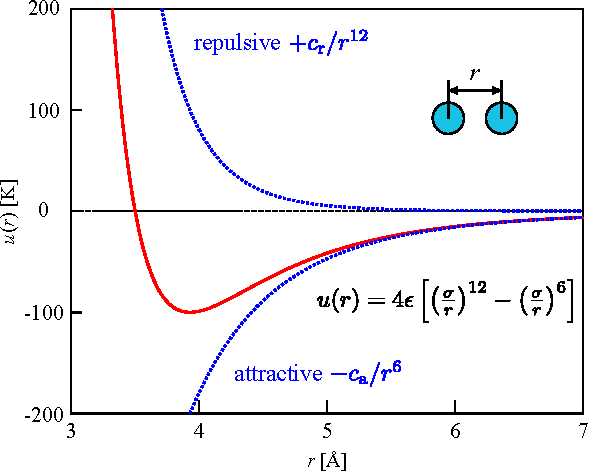
\includegraphics[scale=0.82]{_figure/lj-centre}
\par\end{centering}

\caption[LJ pair potential]{LJ pair potential. The plot gives the potential energy $u(r)$ versus
internuclear distance $r$ of two particles. At large distances, both
attractive and repulsive interactions are small. As the distance between
the atoms decreases, the attractive electron-proton interactions dominate,
and the energy of the system decreases. At the observed bond distance,
the repulsive electron-electron and proton-proton interactions just
balance the attractive interactions, preventing a further decrease
in the internuclear distance. At very short internuclear distances,
the repulsive interactions dominate, making the system less stable
than the isolated atoms.\label{fig:LJ-pair-potential}}
\end{figure}


The Lennard-Jones (LJ) interaction gives

\begin{equation}
u_{LJ}(r)=4\varepsilon\left[\left(\frac{\sigma}{r}\right)^{12}-\left(\frac{\sigma}{r}\right)^{6}\right]
\end{equation}
where $r$ (of unity {[}$\textrm{\AA}${]}) is the distance from central
to central, $\sigma$ (of unity {[}$\textrm{\AA}${]}) is the collision
diameter is the separation of particles where $u(r)=0$, and $\epsilon$
is the well depth of the potential (of unity $\mathrm{kJ/mol}$).
This well (the minimum) occurs at $r_{\min}=2^{1/6}\sigma$ and $u(r_{\min})=-\epsilon$.
The parameters $\sigma$ and $\epsilon$ can be measured by experimentation.

Theoretically, all terms in the multipole series represent attractive
contributions to the potential. The leading term, varying as $r^{-6}$,
describes the dipole-dipole interaction. Higher-order terms represent
dipole-quadrupole ($r^{-8}$), quadrupole-quadrupole ($r^{-10}$)
interactions, and so on, but these are negligible compared to $r^{-6}$.
The short-range interaction is difficult to calculate, and it is defined
as $r^{-12}$ in the LJ model. 

The electrostatic interaction between two charged particles 1 and
2 is described by the Coulomb point charge interaction:
\begin{equation}
u_{\mathrm{Coul}}(r)=\frac{q_{1}q_{2}}{4\pi\varepsilon_{0}r}
\end{equation}


Generally, the pair potential for atomic particles $u(r)$ used is
a sum of LJ and Coulomb interactions.


\subsection{Molecular fluid model}

As discussed before, atomic description of interactions is not sufficient
to well describe solvation properties. For polar liquids, the dipole-dipole
interaction should be mainly taken into account. It can be superposed
onto the spherically symmetric potential:
\begin{equation}
u(1,2)=u_{0}(r)-\boldsymbol{\mu}_{1}\cdot\mathbf{T}(\mathbf{r})\cdot\boldsymbol{\mu}_{2}
\end{equation}
where $\mathbf{r}$ is the vector separation of the molecular centers,
$u_{0}(r)$ is the spherically symmetric term as discussed above,
$\boldsymbol{\mu}_{i}$ is the dipole moment vector of particle $i$
and $\mathbf{T}(\mathbf{r})$ is the dipole-dipole interaction tensor:
\begin{equation}
T(\mathbf{r})=\nabla^{2}\left(\dfrac{1}{r}\right)=3\mathbf{r}\mathbf{r}/r^{5}-\mathbf{I}/r^{3}
\end{equation}
where $\mathbf{I}$ is the unit tensor.

The site-site model is a further extension of atomic model, in which
the solvent molecule is represented by a set of discrete interaction
sites. The total potential energy is a sum of spherical interaction
potentials: 
\begin{equation}
u(1,2)=\frac{1}{2}\sum_{\alpha}\sum_{\beta}u_{\alpha\beta}(\left|\mathbf{r}_{2\beta}-\mathbf{r}_{1\alpha}\right|)
\end{equation}
where $\mathbf{r}_{is}$ is the coordinates of site $s$ in molecule
$i$, $u_{\alpha\beta}(r)$ the interatomic potential energy of pair
of sites $\alpha$, $\beta$, as discussed above. This model is the
mostly adopted, as well as in this thesis.

The full formalism of molecular fluid is $u(\mathbf{r}_{12},\mathbf{\Omega}_{1},\mathbf{\Omega}_{2})$
as in eq. (\ref{eq:pair-potential}). It can be without any supplementary
approximation, with in the frame of pair-additive assumption. 


\subsection{Multipole and spherical harmonic expansion}

The molecular model potential is often expanded to multipole, owing
to the fast convergence of $u$ with respect to the expansion order:\marginpar{In this thesis we use \textcolor{red}{???}}
\begin{equation}
u(1,2)=q\mathbf{T}^{(0)}(\mathbf{r})-\boldsymbol{\mu}\cdotp\mathbf{T}^{(1)}(\mathbf{r})+\dfrac{1}{2}\mathbf{Q}\colon\mathbf{T}^{(2)}(\mathbf{r})-\dfrac{1}{6}\mathbf{O}\vdots\mathbf{T}^{(3)}(\mathbf{r})+\ldots
\end{equation}
where $\mathbf{T}^{(l)}(\mathbf{r})=\nabla^{l}\left(\frac{1}{r}\right)$,
and $q$, $\boldsymbol{\mu}$, $\mathbf{Q}$, $\mathbf{O}$ are the
monopole, dipole, quadrupole and octopole moments. \textcolor{red}{(Physical
meaning and magnitude of each term.)} Other forces such as magnetic,
multipolar, dispersion and induction intermolecular forces are usually
negligible compares to the dipole interaction.

The molecular model potential can also be expanded to spherical harmonics:
\begin{equation}
u(1,2)=\sum_{lm}u_{m}^{l}Y_{m}^{l}(\mathbf{\Omega})
\end{equation}
 Potentials of the same order in multipole or \acs{GSH} are mathematically
equivalent to each other. \textcolor{red}{(When $\psi=0$?)}


\subsection{SPC/E water model}

As water can't be perfectly described by the pair potential due to
multi-body effects, quantum effects, hydrogen bond, etc., there develops
various models to fit certain properties. The models contain several
sites, which can be placed elsewhere other than the center of atom
(figure \ref{fig:Water-models}). The more sites the model has, the
more precise it can be. There is a great work done by Martin Chaplin
\citep{water-model}, which summarized all frequent water models. 

\begin{figure}[h]
\begin{centering}
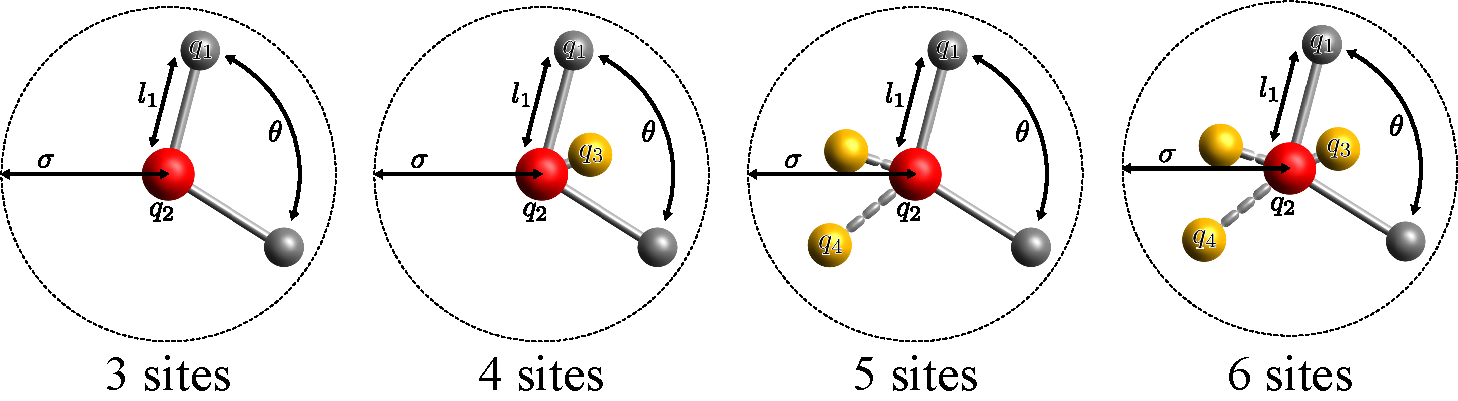
\includegraphics[width=0.75\columnwidth]{_figure/water}
\par\end{centering}

\caption{Water models\label{fig:Water-models}}
\end{figure}


In this thesis, we use the extended simple point charge model (SPC/E)
of water \citep{SPC/E} as the solvent though all this thesis. \marginpar{It should be noted that any rigid solvent model is compatible with
the theory of liquids, e. g. acetonitrile used in \citep{Zhao_2011}.} It is a 3-site model, the electrostatic interaction is modeled using
Coulomb's Law and the dispersion and repulsion forces using the Lennard-Jones
potential.

The SPC/E model adds an polarization correction term to the SPC potential
energy function:

\[
E_{\mathrm{pol}}=\frac{1}{2}\sum_{i}\dfrac{(\mu-\mu^{0})^{2}}{\alpha_{i}}
\]
where $\mu$ is the dipole of the effective pair model, $\mu^{0}$
is the dipole moment of an isolated water molecule, and $\alpha_{i}$
is an isotropic scalar polarizability \citep{SPC/E}. The SPC/E model
gives a better radial distribution function and diffusion constant
than the SPC model, \textcolor{red}{and it is successful in ... (applications)}

The parameters are listed in table \ref{tab:SPC/E}, compared with
its relative SPC model. As the numerical density, dielectric constant,
etc. vary with temperature, we fix the temperature at 298K. \textcolor{red}{(Which
properties needed?)}

\begin{table}[h]
\subfloat[Structural parameters \citep{SPC/E}]{\begin{centering}
\begin{tabular}{lllllll}
\toprule 
\tableheadline{Model} & $\sigma$ $[\lyxmathsym{\AA}^{6}]$ & $\varepsilon$ $[\mathrm{kJ\cdot mol^{-1}}]$ & $l_{1}$ $[\text{\AA}]$ & $q_{1}$ $[e]$ & $q_{2}$ $[e]$ & $\theta$ $[\text{\textdegree}]$\tabularnewline
\midrule
SPC{[}94{]} & 3.166 & 0.650 & 1.0000 & +0.410 & -0.8200 & 109.47\tabularnewline
SPC/E{[}3{]} & 3.166 & 0.650 & 1.0000 & +0.4238 & -0.8476 & 109.47\tabularnewline
\midrule 
experiment{[}90{]} & - & - & 0.991 & - & - & 105.5\tabularnewline
\bottomrule
\end{tabular}
\par\end{centering}

}

\subfloat[Calculated physical properties. All the data is at 25 \textdegree C
and 1 atm.]{\begin{centering}
\begin{tabular*}{1\columnwidth}{@{\extracolsep{\fill}}llllll}
\toprule 
\tableheadline{Model} & \tableheadline{{\footnotesize{}Molar}} & \tableheadline{{\footnotesize{}Number} } & \tableheadline{{\footnotesize{}Dielectric}} & \tableheadline{{\footnotesize{}Dipole}} & \tableheadline{{\footnotesize{}Vapor}}\tabularnewline
 & \tableheadline{{\footnotesize{}Volume {[}$\mathrm{cm^{3}}${]}}} & \tableheadline{{\footnotesize{}Density}} & \tableheadline{{\footnotesize{}Constant}} & \tableheadline{{\footnotesize{}Moment {[}D{]}}} & \tableheadline{{\footnotesize{}Pressure}}\tabularnewline
\midrule
SPC &  &  & 65 {[}185{]} & 2.274\citep{SPC/E} & \tabularnewline
SPC/E &  &  & 71 {[}3{]}\citep{Kusalik_1994_dc_spc/e} & 2.351\citep{SPC/E} & \tabularnewline
\midrule 
experiment & 18.0685 {[}1006{]} &  & 78.4 & 2.95 & 3.165 kPa (25 C) {[}808{]};\tabularnewline
\bottomrule
\end{tabular*}
\par\end{centering}

}\caption{Parameters for SPC and SPC/E water\label{tab:SPC/E}}
\end{table}



\subsection{Flexible and polarizable models}

Flexible models give extra degrees of freedom in vibration and internal
rotation. The interaction potential can contain several terms, typically
about 5 kind of force: the direct interactions (figure ), in addition
to the indirect interactions (LJ and Coulomb).

\begin{figure}[h]
\begin{centering}
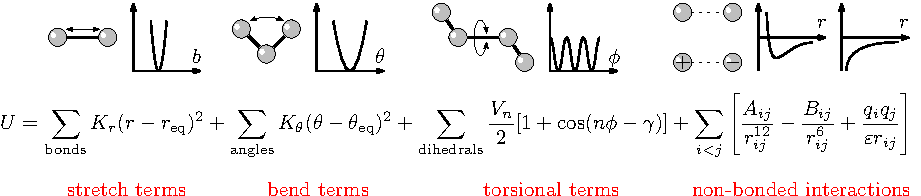
\includegraphics[width=1\columnwidth]{_figure/flexible}
\par\end{centering}

\caption{Direct interactions}
\end{figure}


The flexible model can deal with non-rigidity of solvent, and it partially
polarized owing to the vibration freedom. \textcolor{red}{(Interaction
site model can also deal with non-rigidity of solvent?)}

A rigid model can be polarized by amusing a modifiable charge distribution.
\textcolor{red}{(What else to be added?)}

Complex models require expensive computing cost, but still can have
large fluctuations due to use of small system size. There is a compromise
between the choice of model and the choice of system size. For this
reason, rigid model is now the most popular. On the other hand, computing
technology has largely developed comparing to the theories themselves,
which allows more and more precise models to be used in computation. 


\section{Model of solute}

The model of solute also gives an influence to the energy and structure
of solvation. The compromise to have a better model of solvent or
solute is debatable, and it varies according to the application. For
example, we never use a quantum solvent model in the case of an implicit
solute, since this would not be profitable even if the solute is of
simple geometry (wall). On the other hand, Most of \acs{QM} calculations
in apolar solvents (toluene, etc.) use implicit SCRF model, or even
without solvent correction, and this has been proven to work well.
In the case of molecular solutes, we generally require the solute
to have at least a model at the same scale of description (figure
\ref{fig:Hierarchy-of-models}).

\begin{flushright}
\begin{figure}[h]
\centering{}%
\begin{minipage}[t]{1\columnwidth}%
\begin{center}
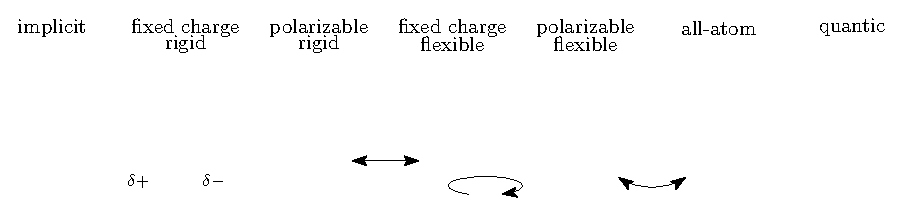
\includegraphics[width=1\columnwidth]{_figure/solute}
\par\end{center}%
\end{minipage}\caption{Hierarchy of models\label{fig:Hierarchy-of-models}}
\end{figure}

\par\end{flushright}

In this thesis, we use also rigid model to describe solute to be coherent
with IET, which cannot treat the solvent and solute in different scale
of description. Polarizable, flexible model of solute, and coupling
with QM will be described in perspective.

In a word, the choice of the model of system is a compromise between
the required precision according to application, and the computing
cost that the research can afford.
